

\newif\ifinria
\def\ptitle{EB-Net for landmarking on pronotum images} % Title
\def\pauthor{Le Van Linh} % Author
\def\padvisors{Beurton-Aimar Marie, Zemmari Akka, Parisey Nicolas} % Advisors
\def\pteam{I\&S Team} % Team
\def\pinstitute{Univ. Bordeaux, LaBRI, France} % Affiliation
\def\pdate{Thursday April 4, 2019} % Date
% \inriatrue % inriatrue/inriafalse to enable/disable Inria logo
\makeatletter
\newcommand*{\rom}[1]{\expandafter\@slowromancap\romannumeral #1@}
\makeatother


\pdfobjcompresslevel=0
\documentclass[final,hyperref={pdfpagelabels=false},table]{beamer}
\usepackage[orientation=portrait,size=a0,scale=1.4]{beamerposter}
\usepackage[utf8]{inputenc}
\usepackage[sfdefault]{roboto}
\usepackage[english]{babel}
\usepackage{amsmath, amsthm, amssymb, array, booktabs, grffile, latexsym, tabularx, xspace}
\newcolumntype{Z}{>{\centering\arraybackslash}X}
\newcommand{\pphantom}{\textcolor{ta3aluminium}}
\newlength{\columnheight}

\def\plogo{logo/logo_LaBRI.png}
\def\purl{https://www.labri.fr/}
\def\pmail{Twitter: @labriOfficial}

\mode<presentation>{\usetheme{SDSLaBRI}}
\title[\ptitle]{\texorpdfstring{\huge \ptitle}{\ptitle}}
\author[\pauthor]{\pauthor\ -\ \padvisors}
\institute[\pinstitute]{\pteam\ -\ \pinstitute}
\date[\pdate]{\pdate}
\setlogo{\plogo}
\setauthorurl{\purl}
\setauthoremail{\pmail}

\graphicspath{{./fig/}} % Figures and logos directory
\setlength{\columnheight}{25.1cm} % Tweak this value if columns are too long/short (should be okay with 588ex)

\usepackage{multicol}
\usepackage{ragged2e}
\usepackage{times} % Use the times font
\usepackage{booktabs} % Top and bottom rules for table
\usepackage{caption} % Required for specifying captions to tables and figures
\usepackage{amsfonts, amsmath, amsthm, amssymb} % For math fonts, symbols and environments
\usepackage{booktabs}
\usepackage{multirow}
\apptocmd{\thebibliography}{\footnotesize \justifying\hyphenchar\font=-1}{}{} 
\usepackage{tabu} 
\usepackage{xcolor}    
      
%\setlength{\arrayrulewidth}{1mm}
\renewcommand{\arraystretch}{1.2}
\definecolor{myyellow}{RGB}{255, 191, 0}

\begin{document}
\begin{frame}
  \begin{columns}
    \begin{column}{.53\textwidth}
      \begin{beamercolorbox}[center,wd=\textwidth]{postercolumn}
        \begin{minipage}[T]{.95\textwidth}
          \parbox[t][\columnheight]{\textwidth}{
            \begin{block}{Context}
            	\begin{itemize}
            		\item \textbf{Deep learning}\cite{lecun2015deep}: methods to learn the representations of data.
            		\item \textbf{Landmarks} (key points): the points on the image that are invariant when the image changes.
             		\item \textit{Key points detection}: to find the key points through images.
             		\item Landmarks in biology: most often provided manually by biologists.
            	\end{itemize}
            \end{block}
            
            \vfill            
            \begin{block}{Beetle's pronotum and landmarks}
            \begin{itemize}
            	\item Pronotum: an external morphology part of beetle
            	\item Eight-manual landmarks: provided by biologists and used as ground truth.
            \end{itemize}
            \centering
            
            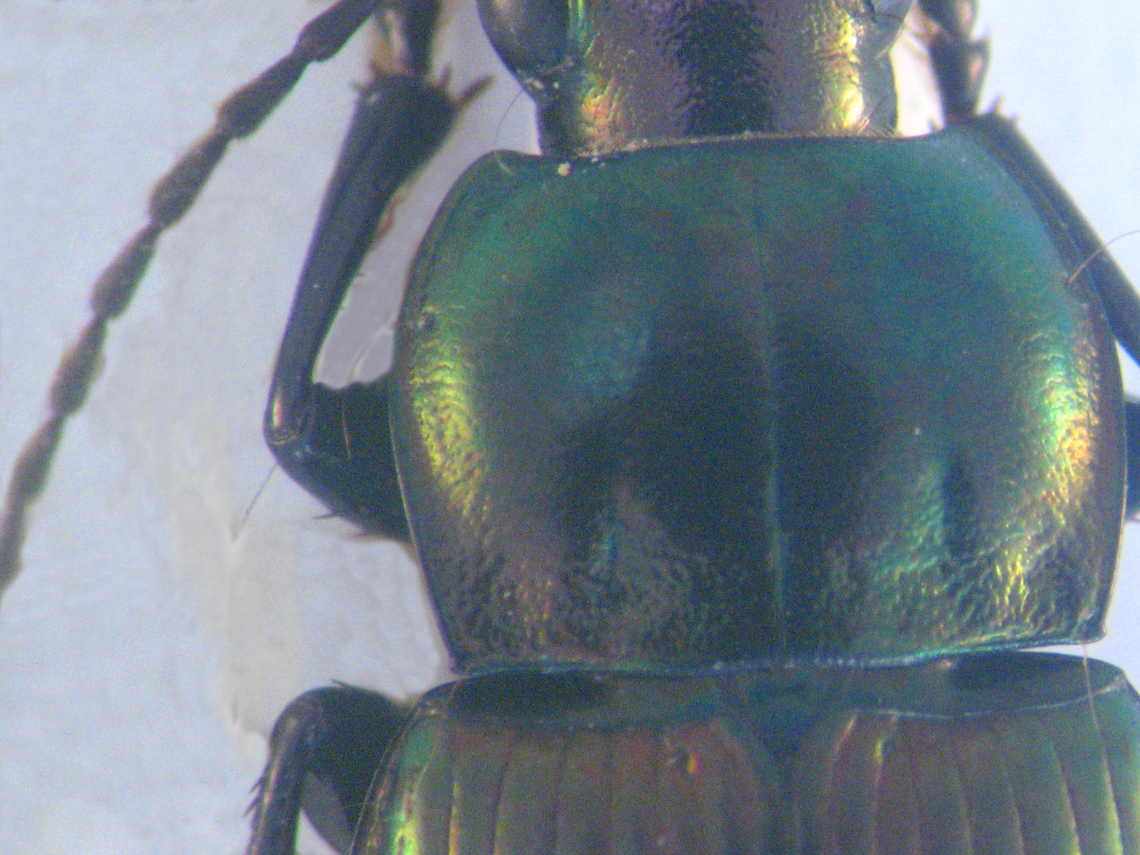
\includegraphics[width=.35\textwidth]{images/pronotum.JPG}~~
            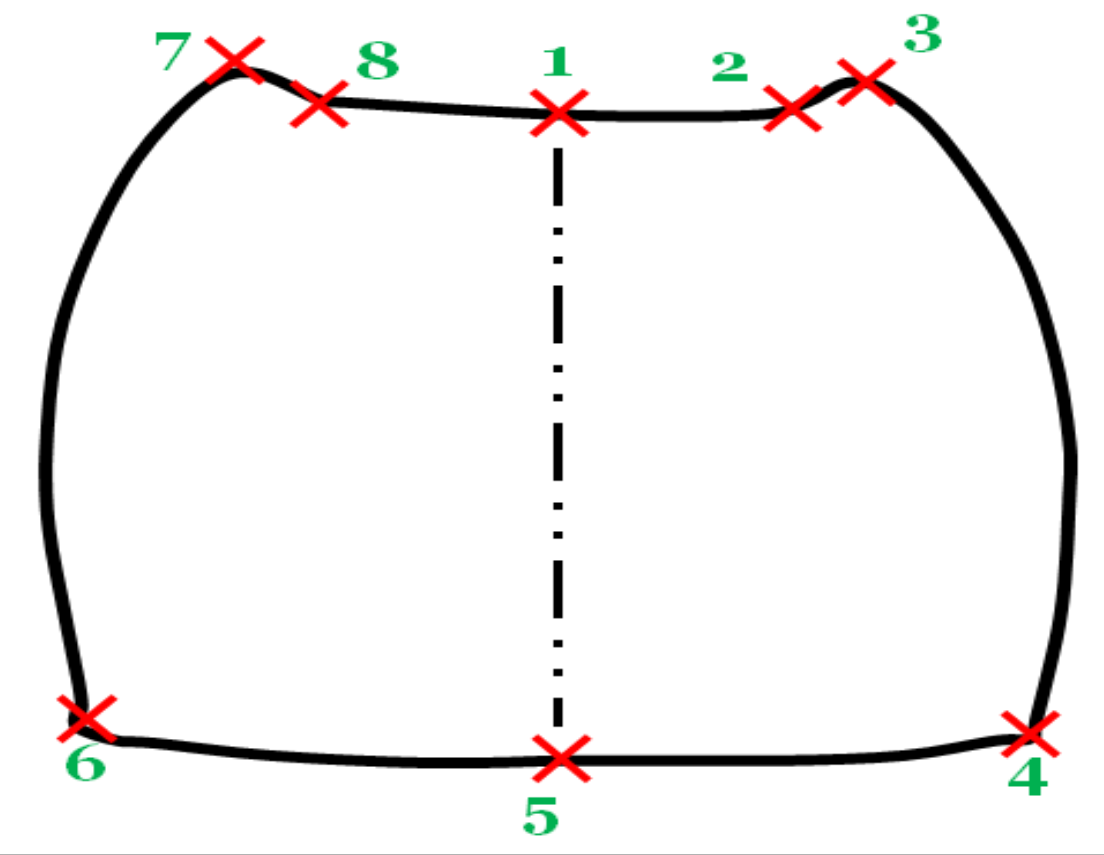
\includegraphics[width=.35\textwidth]{images/pronotum.png}            \\[0.2cm]
            \textbf{\textcolor{red}{How to locate the landmarks automatically?}}
            \end{block}
            
            \vfill            
            \begin{block}{Dataset augmentation}
            	\begin{itemize}
            		\item[] The augmentation includes two procedures:
            			\begin{enumerate}
            				\item Changing the value of one color channel in the original image
            				\item Separating the channels of original image	
			           	\end{enumerate}
					\item[] In total: $293 \times 7 = \textbf{2051}$ images 
            	\end{itemize}
            \centering
            
            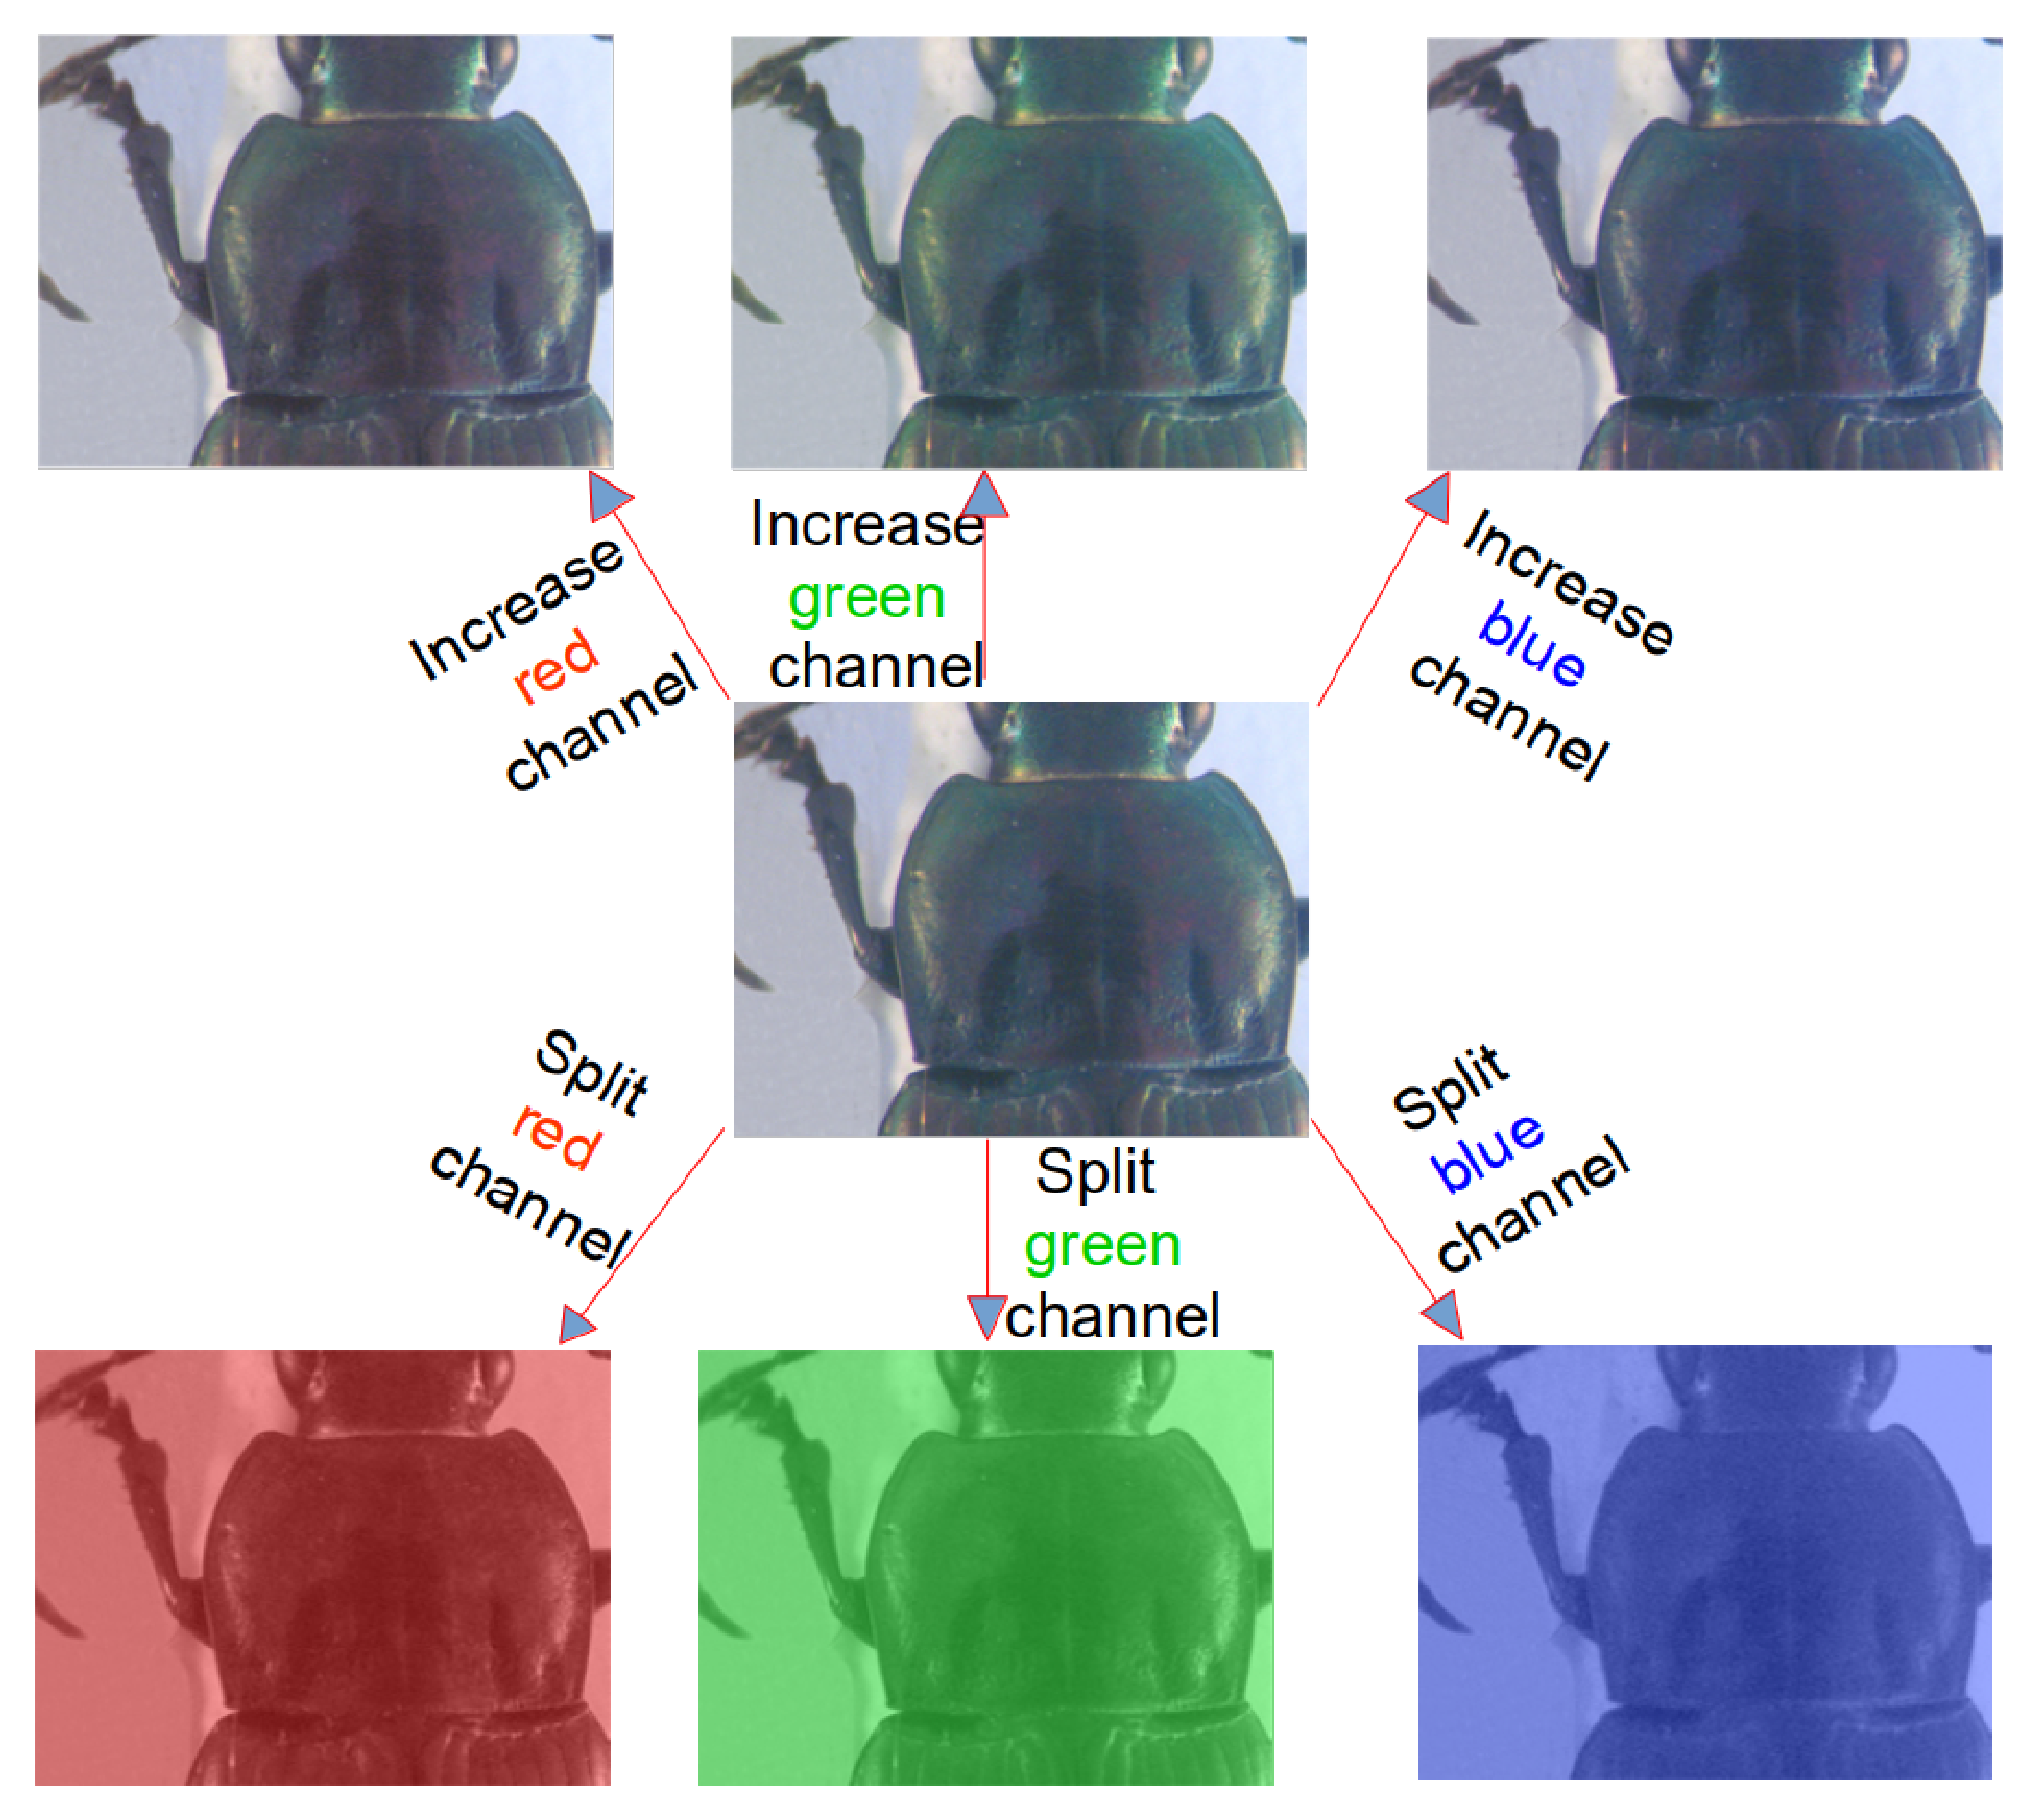
\includegraphics[width=.5\textwidth]{images/data_aug.eps}
            \end{block}
            
            \vfill            
            \begin{block}{Elementary block}
            	\begin{columns}
            		\begin{column}{.45\textwidth}
            			An elementary block (EB) is consists of:
            			\begin{itemize}
            				\item A Convolutional layer
            				\item A Max-Pooling layer
            				\item A Dropout layer
            			\end{itemize}
            		\end{column}
            		\begin{column}{.44\textwidth}
            			\centering
            			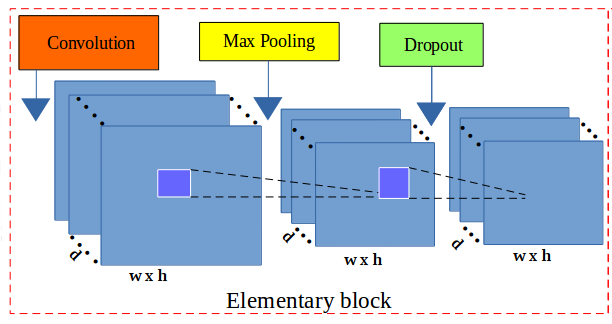
\includegraphics[width=.85\textwidth]{images/elementary_block.png}
            		\end{column}
            	\end{columns}
            \end{block}
            
            \vfill            
            \begin{block}{New model: EB-Net}
            	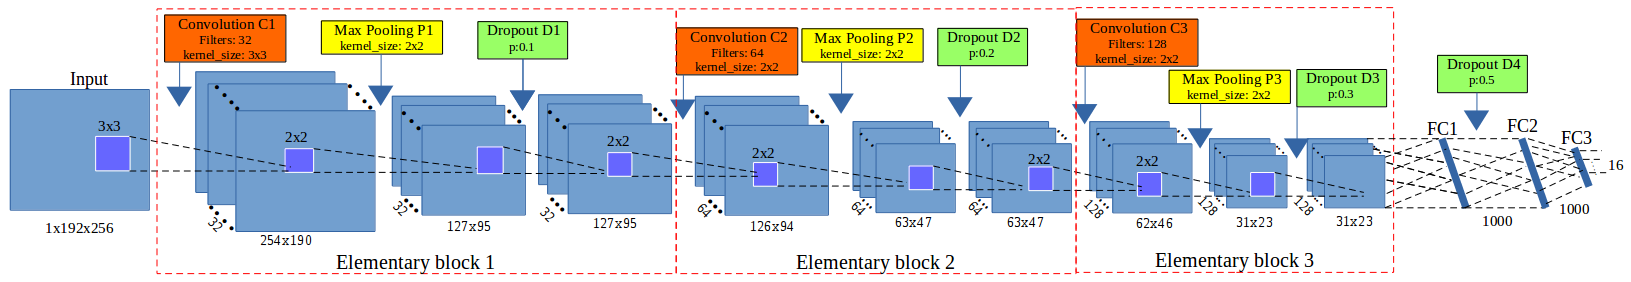
\includegraphics[width=.90\textwidth]{images/arch_model.png}
            The proposed network includes:
            \begin{itemize}
            	\item Three elementary blocks
            	\item Three fully connected layers
            	\item A Dropout layer
            \end{itemize}
            \end{block}
  
          }
        \end{minipage}
      \end{beamercolorbox}
    \end{column}
     
    
    \begin{column}{.53\textwidth}
      \begin{beamercolorbox}[center,wd=\textwidth]{postercolumn}
        \begin{minipage}[T]{.95\textwidth}
          \parbox[t][\columnheight]{\textwidth}{
            
            \begin{block}{Predicted landmarks on images}
            	\begin{itemize}
            		\item \textbf{\textcolor{myyellow}{Yellow}} points are manual landmarks
            		\item \textbf{\textcolor{red}{Red}} points are predicted landmarks
            	\end{itemize}
            	\begin{columns}
            		\begin{column}{.45\textwidth}
            			\centering
            			
\includegraphics[width=.90\textwidth]{images/Prono_115.eps}
            		\end{column}
            		\begin{column}{.45\textwidth}
            			\centering
            			
\includegraphics[width=.90\textwidth]{images/Prono_036.eps}
            		\end{column}
            	\end{columns}
            \end{block}
            
            \vfill
            
            \begin{block}{Evaluation}
            On \textbf{quality metrics} for regression problems.
            \begin{center}            	
           		\begin{tabu} to 0.99\textwidth {| X[c] | X[c] | X[c] | X[c] |}
            		\hline
            		Metric & $r^2$ & EV & Pearson \\ \hline
            		Cintas et al.\cite{cintas2016automatic} & 0.884 & 0.951 & 0.976 \\ \hline                 		    		\rowcolor{green!80!yellow!50} Our model & \textbf{0.9952} & \textbf{0.9951} & \textbf{0.9974} \\ \hline
            	\end{tabu}            
            \end{center}
            On \textbf{average distances} between landmarks (manual \& predicted)
            \begin{center}
           		\begin{tabu} to 0.7\textwidth{| X[c] | X[c] |}
            		\hline
            		\textbf{Landmark} & \textbf{Distance} (in pixels)\\ \hline
            		\rowcolor{red!80!yellow!50} \textbf{\textcolor{blue}{1}} & \textbf{\textcolor{blue}{4.002}} \\ \hline
            		2 & 4.483 \\ \hline
            		3 & 4.296 \\ \hline
            		4 & 4.387 \\ \hline
            		5 & 4.293 \\ \hline
            		\rowcolor{green!80!yellow!50} \textbf{\textcolor{red}{6}} & \textbf{\textcolor{red}{5.363}} \\ \hline
            		7 & 4.636 \\ \hline
            		8 & 4.936 \\ \hline
            	\end{tabu}            
            \end{center}
            The proportion of acceptable predicted landmarks:
	            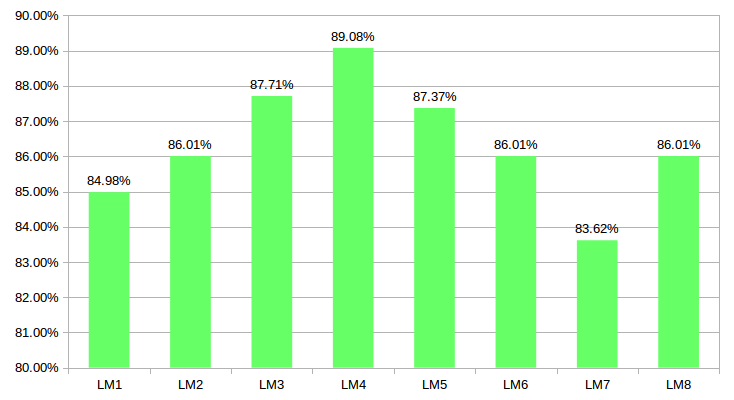
\includegraphics[width=.80\textwidth]{images/chart2.png}
              
            \end{block}
            
            \vfill
            
            \begin{block}{Conclusion}
				\begin{enumerate}
					\item A CNN model has been proposed to predict the landmarks on pronotum images.
					\item An original method has been applied to augment dataset.
					\item The quality of predicted landmarks have been evaluated by average distances with an accuracy greater than $80\%$.
					\item The predicted landmarks can be used to replace manual landmarks.
				\end{enumerate}				            
            \end{block}
            
            \vfill
            
            \begin{block}{Bibliography}
            	\footnotesize{
            	\setbeamertemplate{bibliography item}{\insertbiblabel}
            	\bibliographystyle{unsrt}
				\bibliography{references}
				
				}
            \end{block}
             
          }
        \end{minipage}
      \end{beamercolorbox}
    \end{column}
  \end{columns}
  \vskip1ex
\end{frame}
\end{document}
